\todo{There should be a link either here or at end of literature which forms the basic for different methods (clustering, routing, trip generation).}
\todo{Paragraph describing different types of algorithm used (Routing then cluster, Cluster then Routing, Genetic, etc.)}
\todo{Remember to justify the choice of algorithms. You may also need to explain how to adopt these algorithms in your work. A figure showing the ralationship between different components of your work may also help.}
\todo{Include code for evaluating a route here.}

\subsection{Clustering}\label{subsec:clustering}
Clustering as a concept can be described as `the unsupervised classification of patterns (observation, data items, or
feature vectors) into groups (clusters)'\todo{cite Data Clustering: A review, A.K. Jain}.
In our problem, clustering will be used to group locations together to form an itinerary for each day of the trip.
These clusters, or days, will then be used as an input for some routing algorithm, which will try and find an
optimal route for each day.
These routes can then be combined to form a complete route for the trip.
The goal of our clustering algorithms is to find a set of clusters that, when combined with some routing algorithm,
will produce a route that minimises the cost function.\\
The code below shows how we can use a set of clusters alongside our graph and duration inputs to find a route:
\begin{figure}[H]\label{fig:Clustering.find_route_from_clusters}
    \centering
    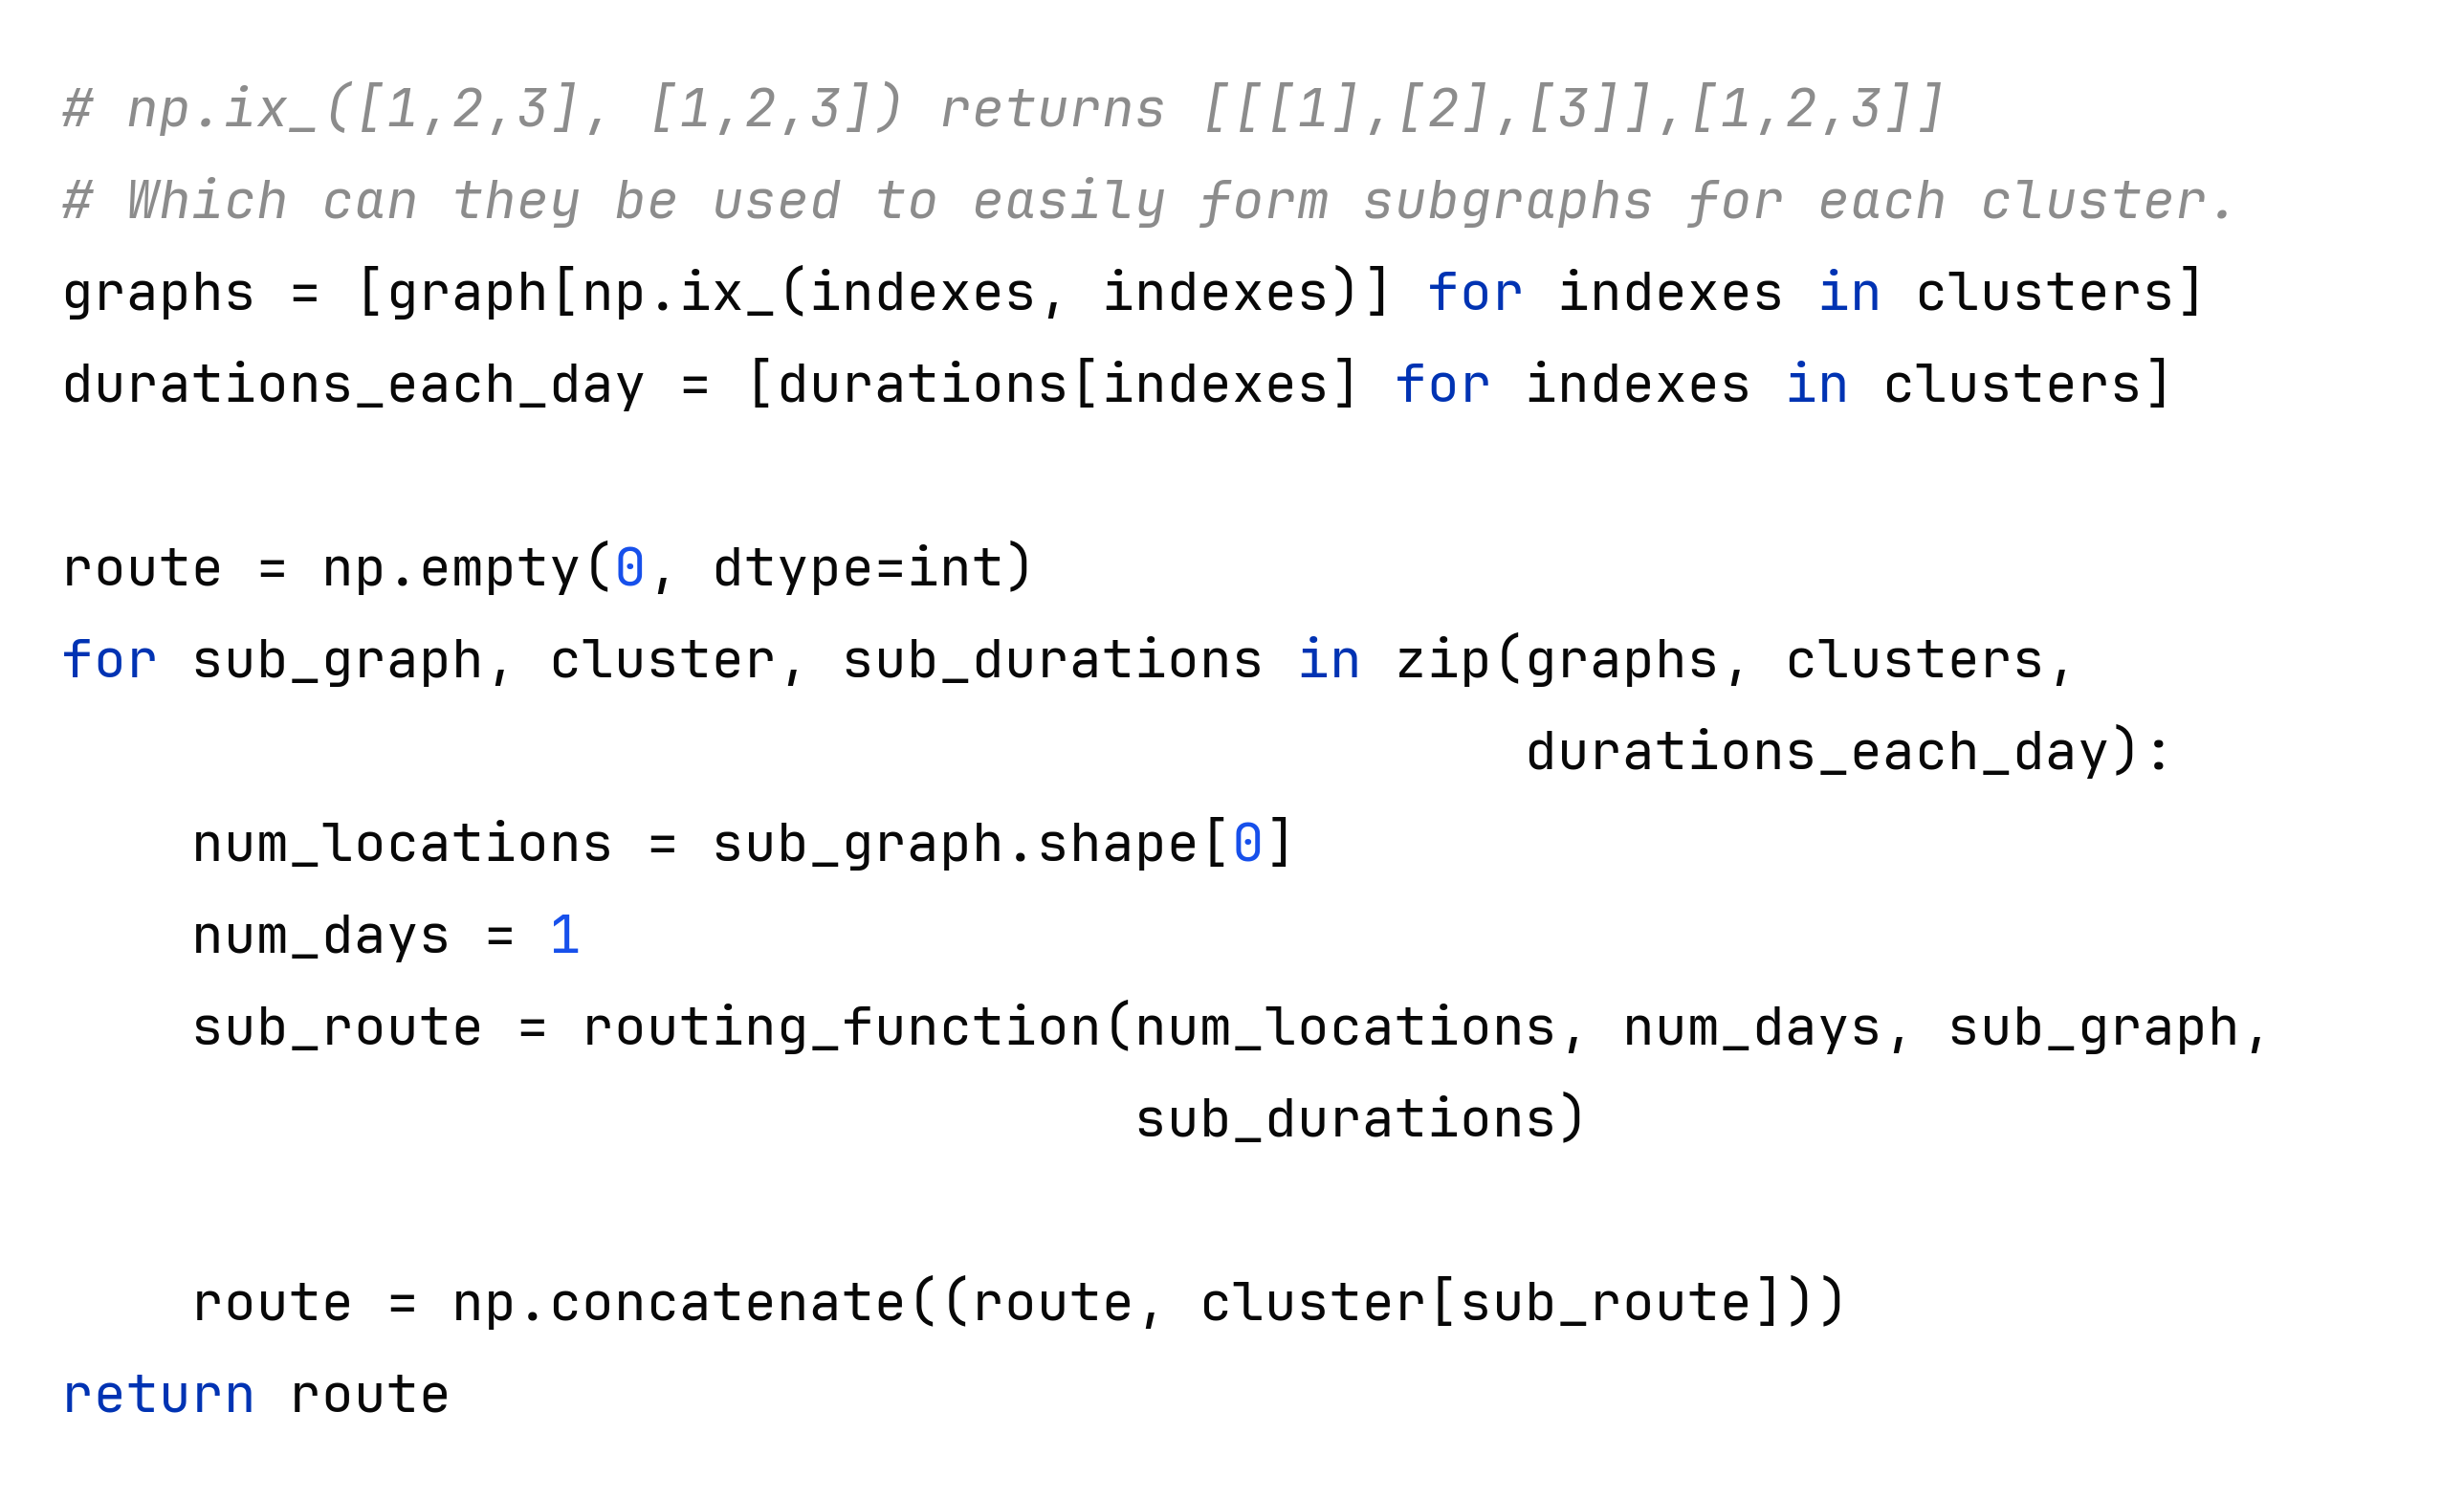
\includegraphics[width = \textwidth]{Clustering.find_route_from_clusters}
    \caption{From Clustering.find\_route\_from\_clusters in algorithms\textbackslash clustering.py}
\end{figure}

\noindent
The clustering algorithms implemented in this project are: K-Means, Genetic Clustering and Genetic Centroid-based
Clustering.

\subsubsection{K-Means}\label{subsubsec:k-means}
K-Means is an iterative clustering algorithm that defines its clusters using a set of centroids (means) which are
given a location in the input space, a given location is assigned to the cluster of the `closest' centroid.
The algorithm starts by initialising random centroids and iteratively improving the clustering from there, continuing
until the algorithm converges (on a local optimum) or an iteration limit is reached.
While the algorithm may not find the best solution, it is rather quick, with a time complexity of $O(mnki)$,
where where $m$ is the number of locations, $n$ is the dimensionality of the input, $k$ is the number of clusters,
and $i$ is the number of iterations iterations\todo{cite Algorithm AS 136: A K-Means Clustering Algorithm}.
Our inputs will always contain only two dimensions, and we will be setting a maximum number of iterations, this
makes both $n$ and $i$ constants allowing us to simplify the time complexity to $O(mk)$.\\

\noindent
In our implementation of K-Means we will initialise our centroids by randomly selecting unique locations from our
input, and placing our centroids at their coordinates.
A different approach was considered, which involved initialising the centroids with random coordinates in a similar
area to the input, however this had the potential to create clusters with zero locations assigned to them resulting
in invalid trips.
By starting with locations from the input, we can be sure that all clusters have at least one location assigned to them.
We will be using the coordinates of our locations to calculate the Euclidean distances between locations and centroids,
these locations will be assigned to the cluster of the closest centroid:
\begin{figure}[H]\label{fig:Clustering._assign_nodes_to_centroid}
    \centering
    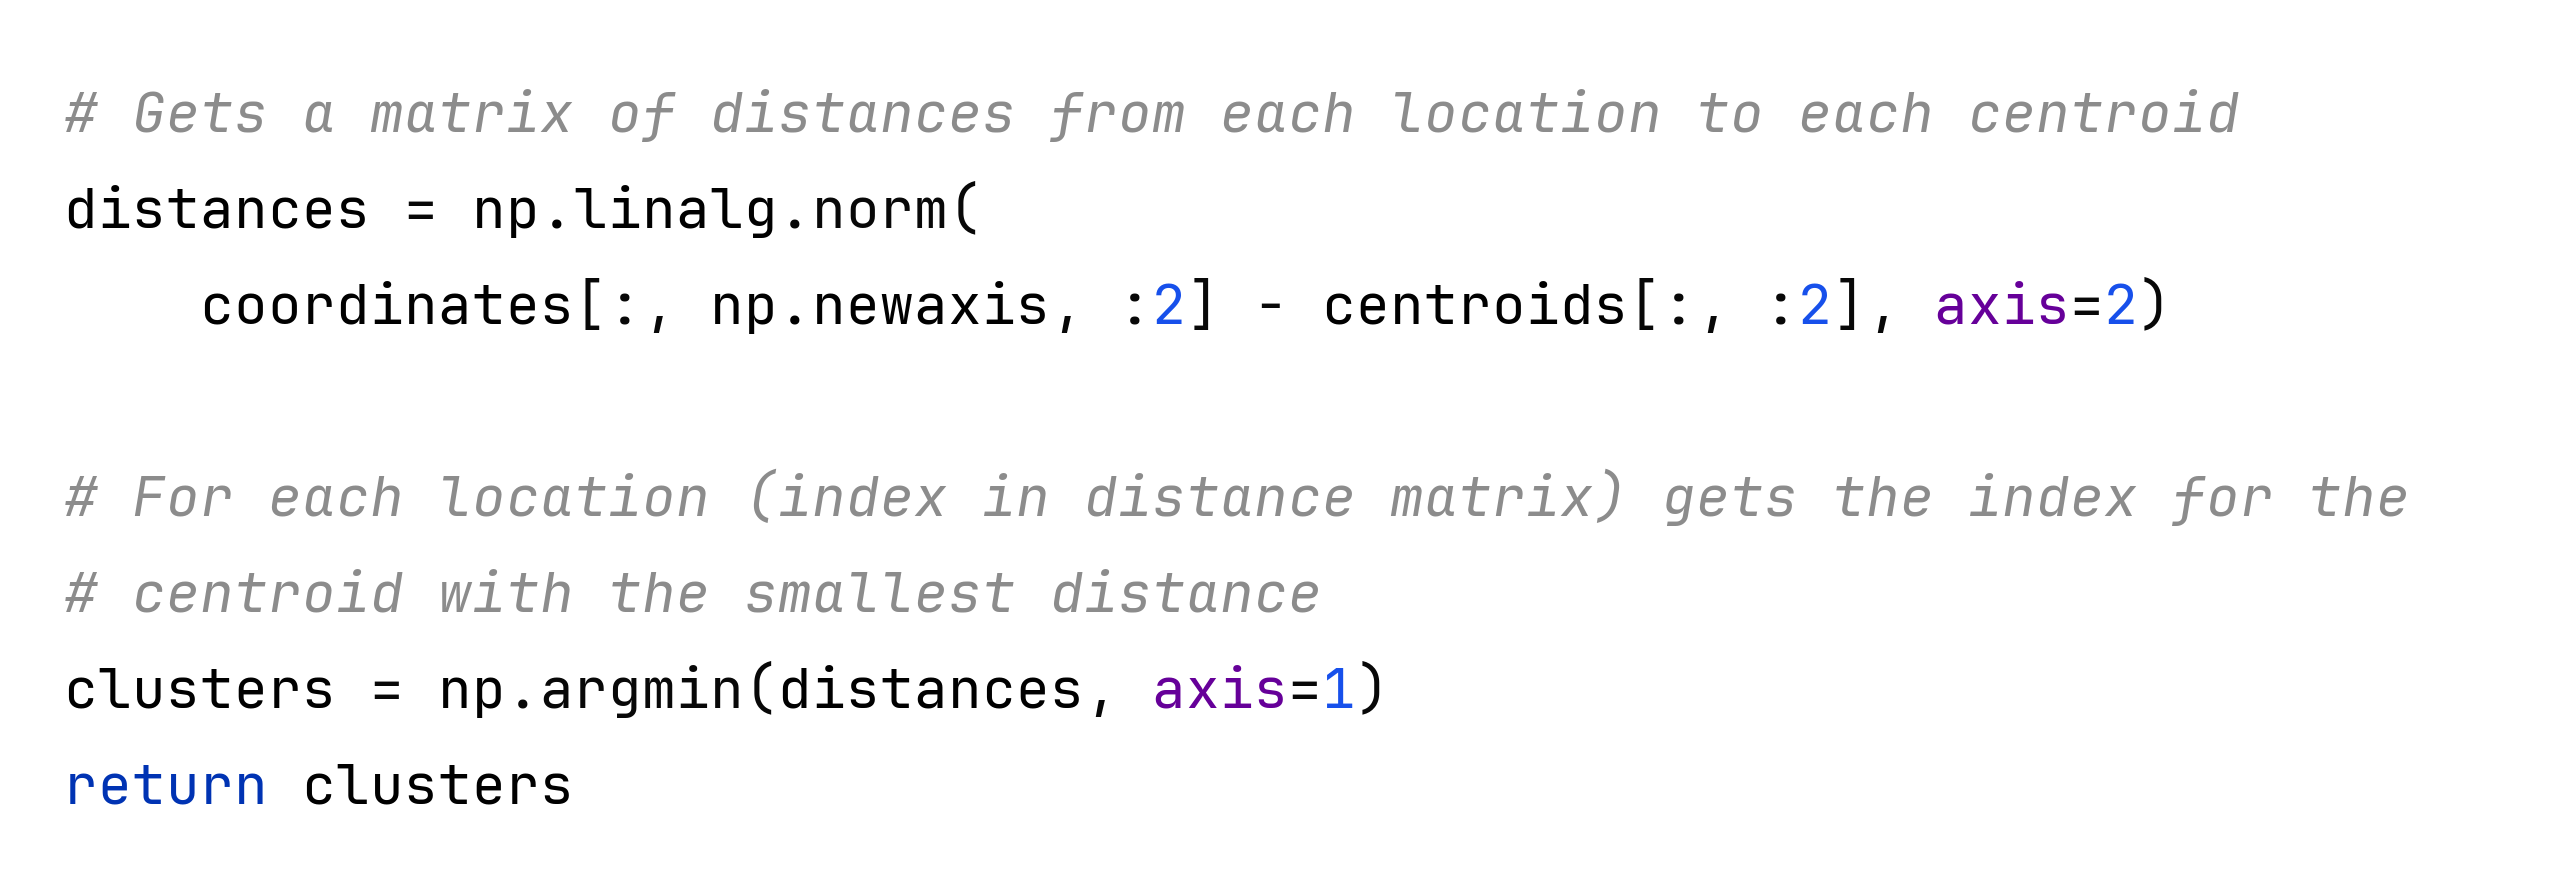
\includegraphics[width = \textwidth]{Clustering._assign_nodes_to_centroid}
    \caption{from Clustering.\_assign\_nodes\_to\_centroid in algorithms\textbackslash clustering.py}
\end{figure}

\noindent
After assignment, the centroids are recalculated such that their coordinates are the average of all locations
assigned to their cluster:
\begin{figure}[H]\label{fig:KMeans._compute_means}
    \centering
    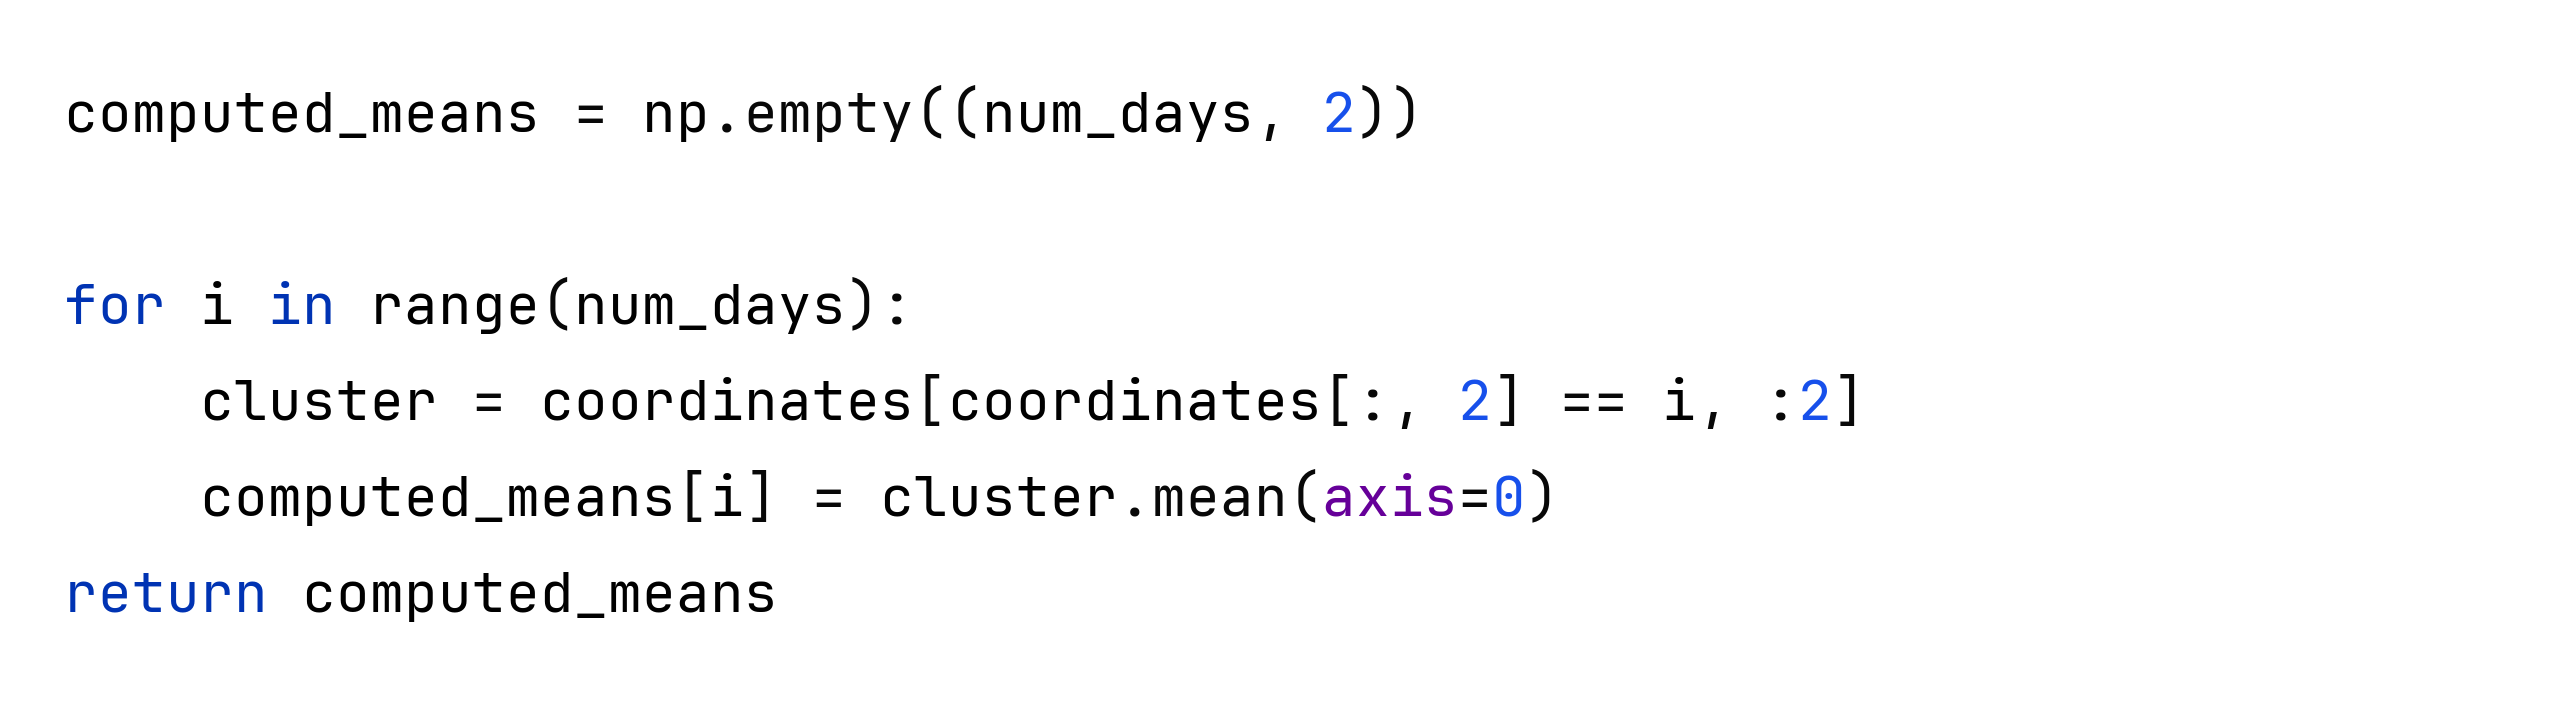
\includegraphics[width = \textwidth]{KMeans._compute_means}
    \caption{from KMeans.\_compute\_means in algorithms\textbackslash clustering.py}
\end{figure}

\noindent
These steps of cluster assignment and centroid recalculation are repeated until either a maximum allowed number of
iterations is reached, or until the algorithm converges on an optimum solution.
Our convergence criterion is that the centroids stop changing between iterations, i.e., the centroids are the same
as the previous iteration:
\begin{figure}[H]\label{fig:KMeans.find_clusters}
    \centering
    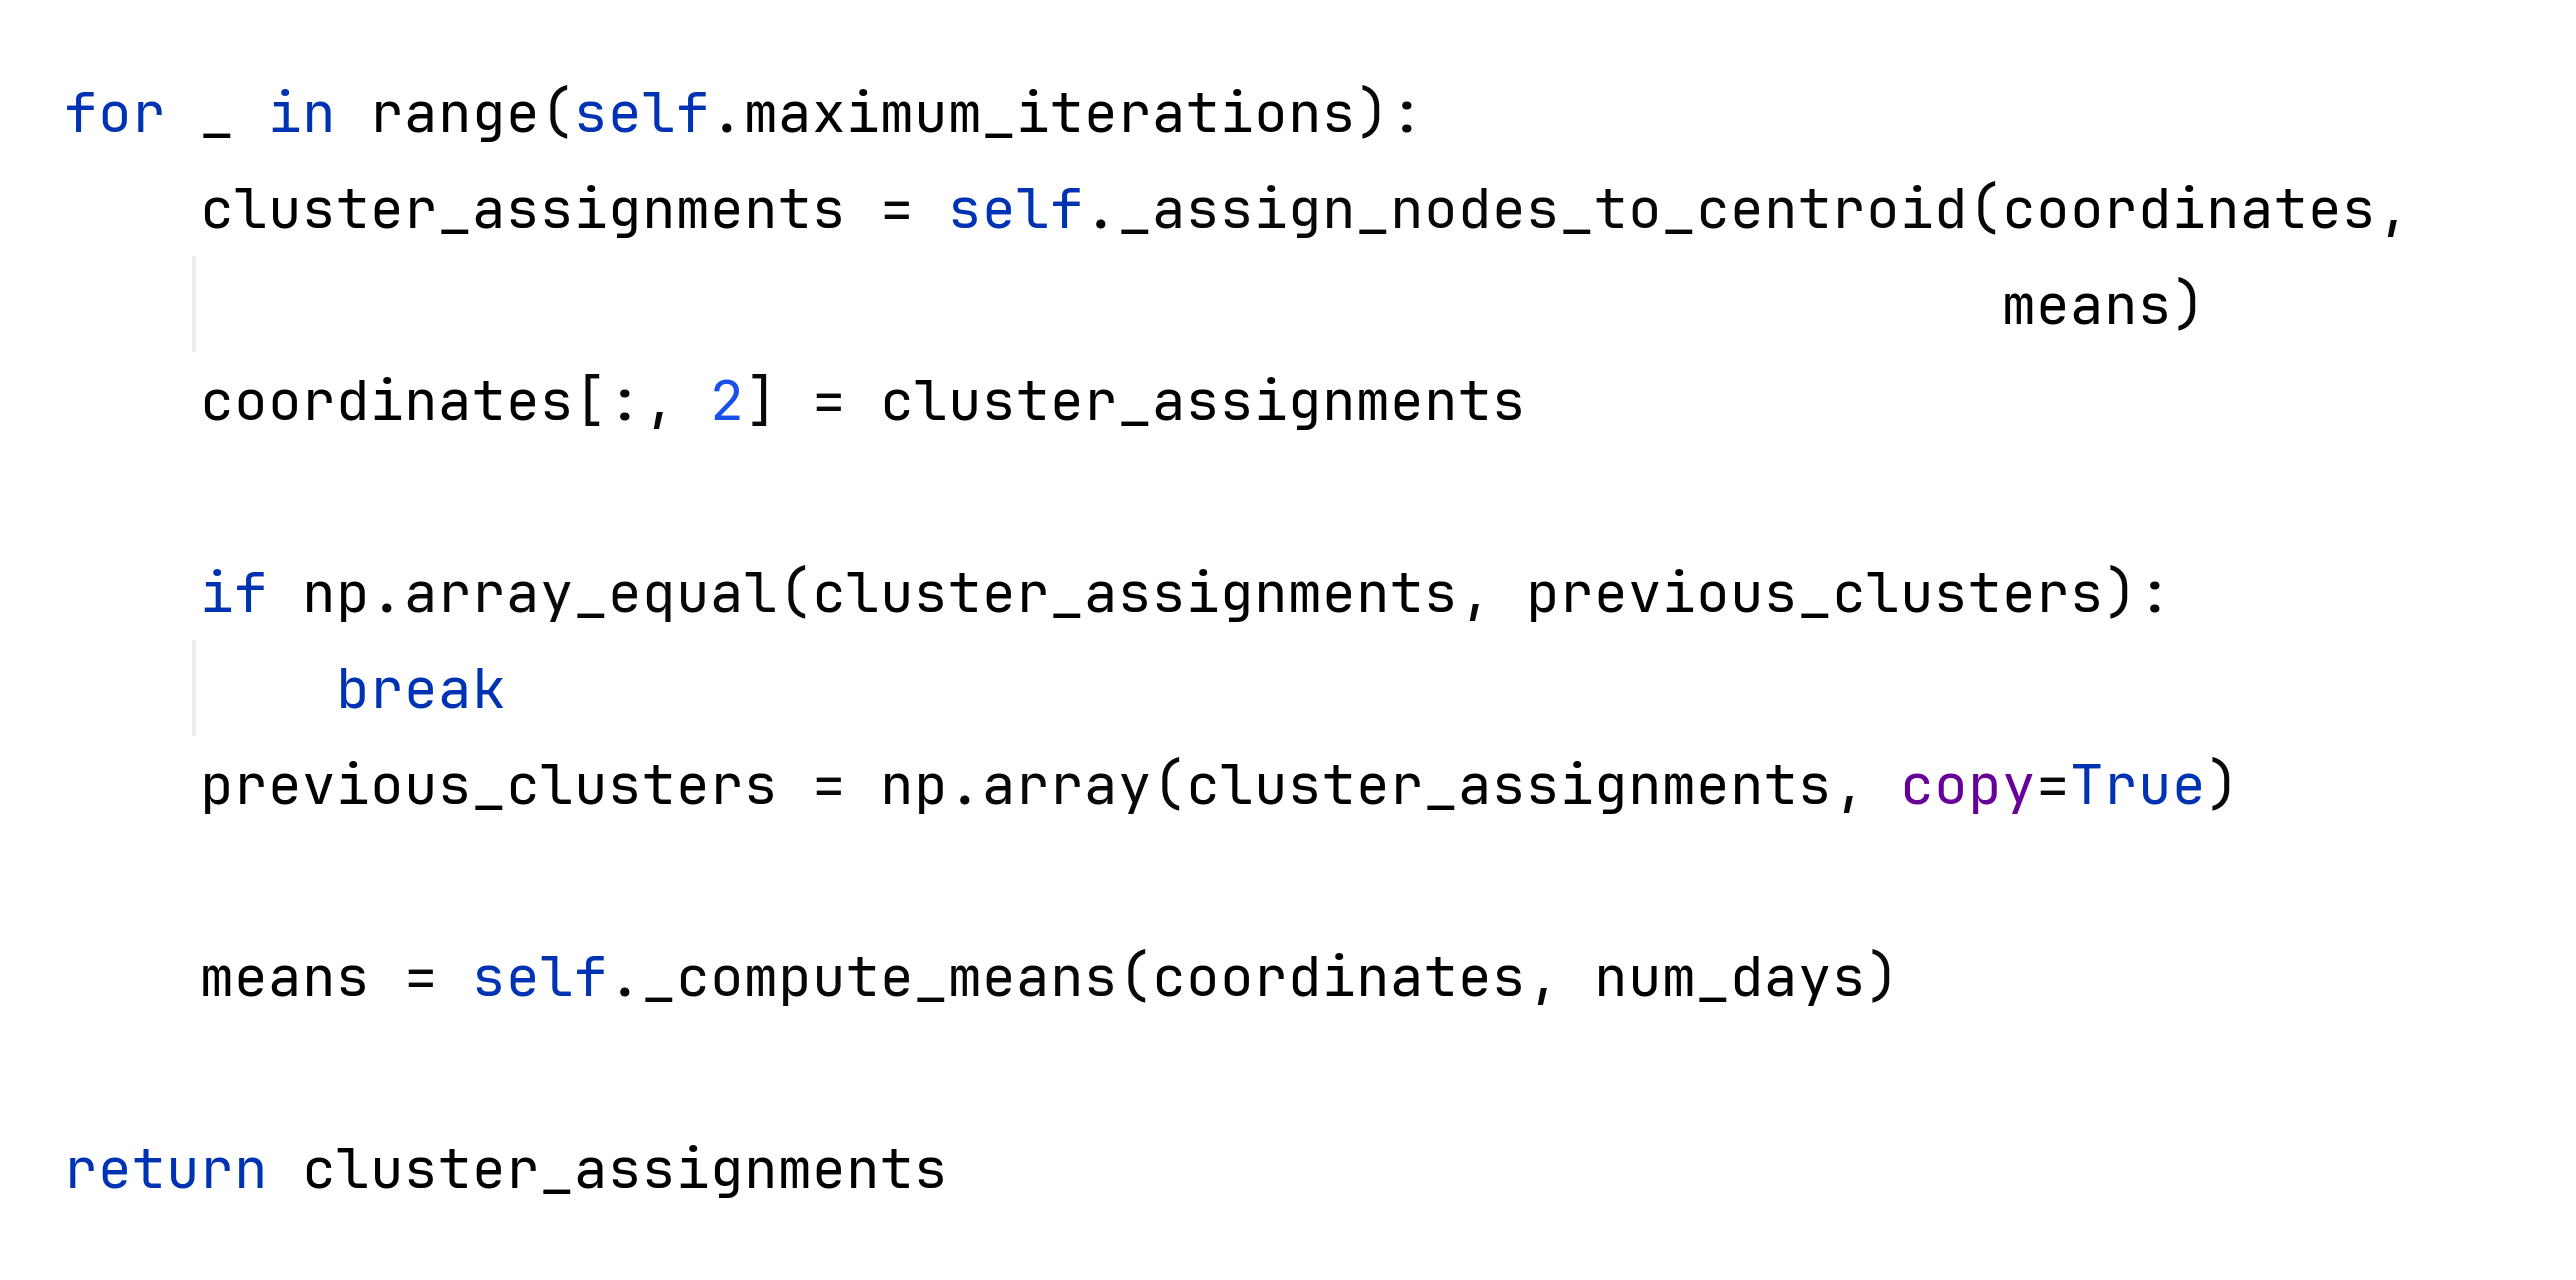
\includegraphics[width = \textwidth]{KMeans.find_clusters}
    \caption{from KMeans.find\_clusters in algorithms\textbackslash clustering.py}
\end{figure}

\noindent
Below is an example of the K-Means algorithm run on an input with 25 points of interest around London over seven days:
\begin{figure}[H]\label{fig:KMeans_London_Step1}
    \ContinuedFloat*
    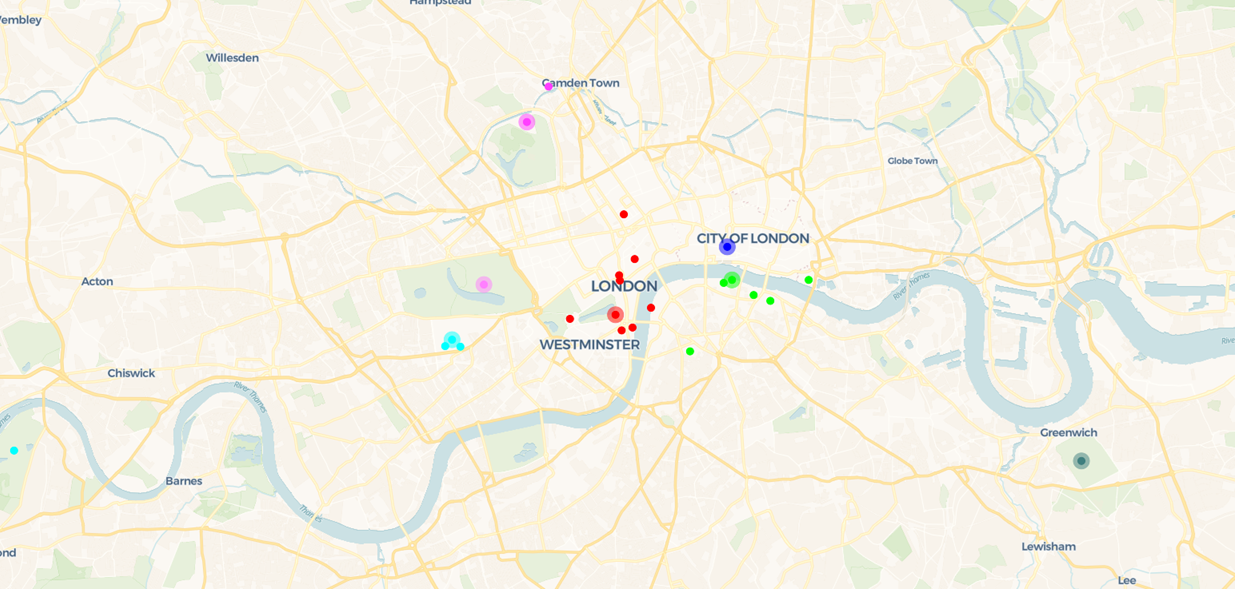
\includegraphics[width = \textwidth]{KMeans_London_Step1}
    \caption{Step 1, Initial centroid positions and cluster assignments.}
\end{figure}
\begin{figure}[H]\label{fig:KMeans_London_Step2}
    \ContinuedFloat
    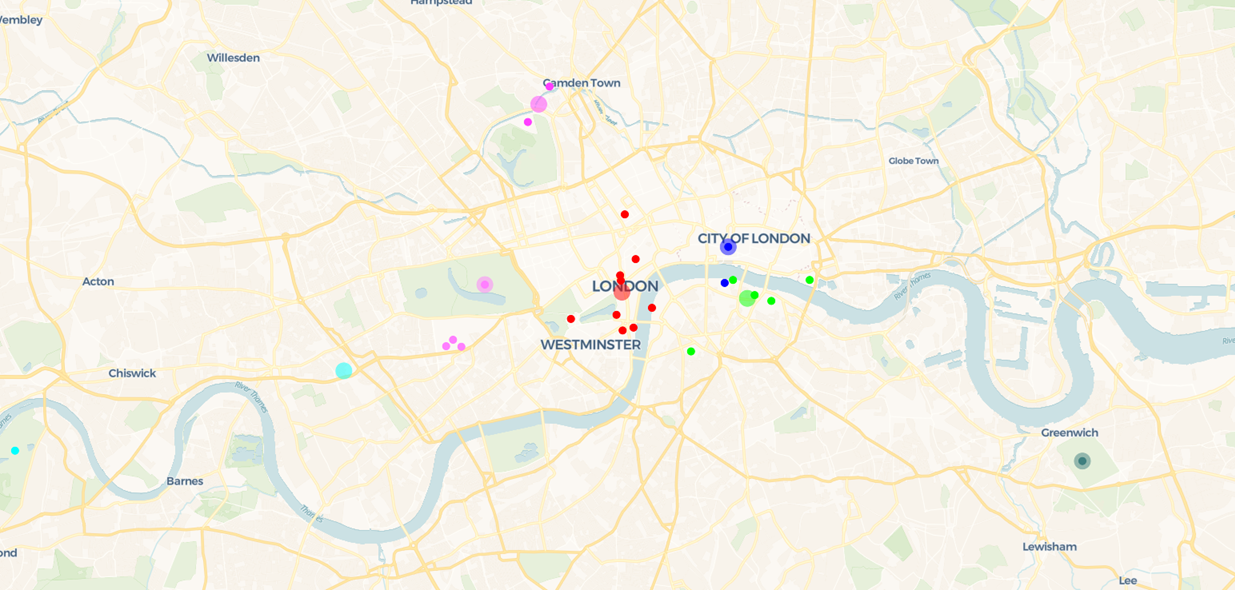
\includegraphics[width = \textwidth]{KMeans_London_Step2}
    \caption{Step2, Centroids have been updated, locations are reassigned to their closest centroid.}
\end{figure}
\begin{figure}[H]\label{fig:KMeans_London_Step3}
    \ContinuedFloat
    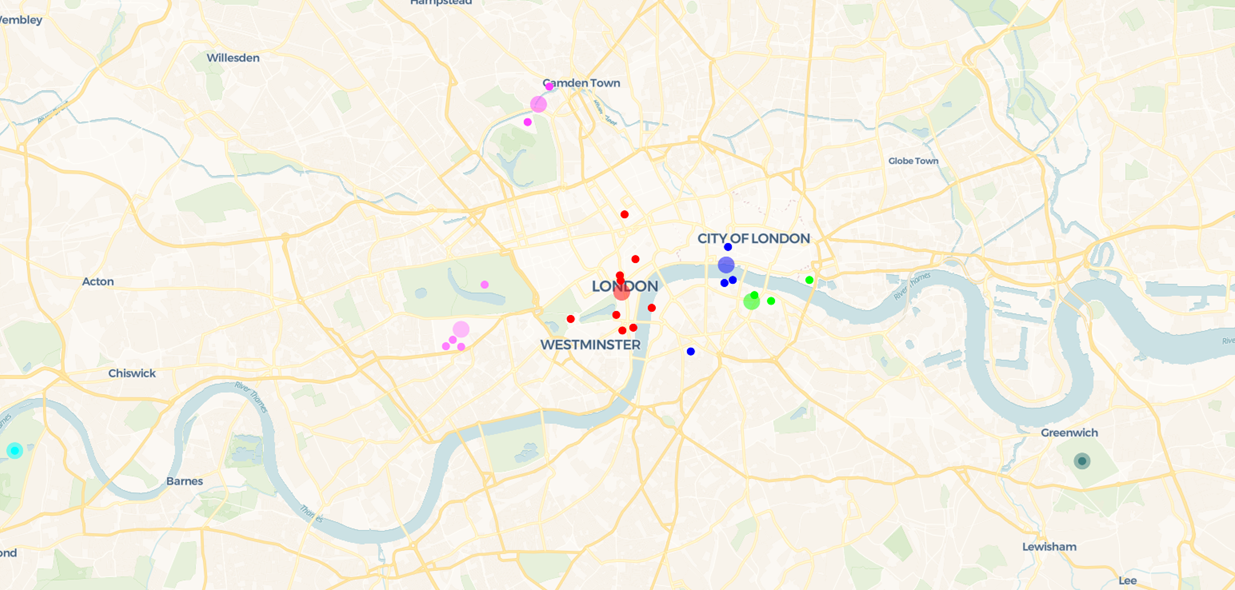
\includegraphics[width = \textwidth]{KMeans_London_Step3}
    \caption{Step3, Centroids updated again and locations updated.}
\end{figure}
\begin{figure}[H]\label{fig:KMeans_London_Step4}
    \ContinuedFloat
    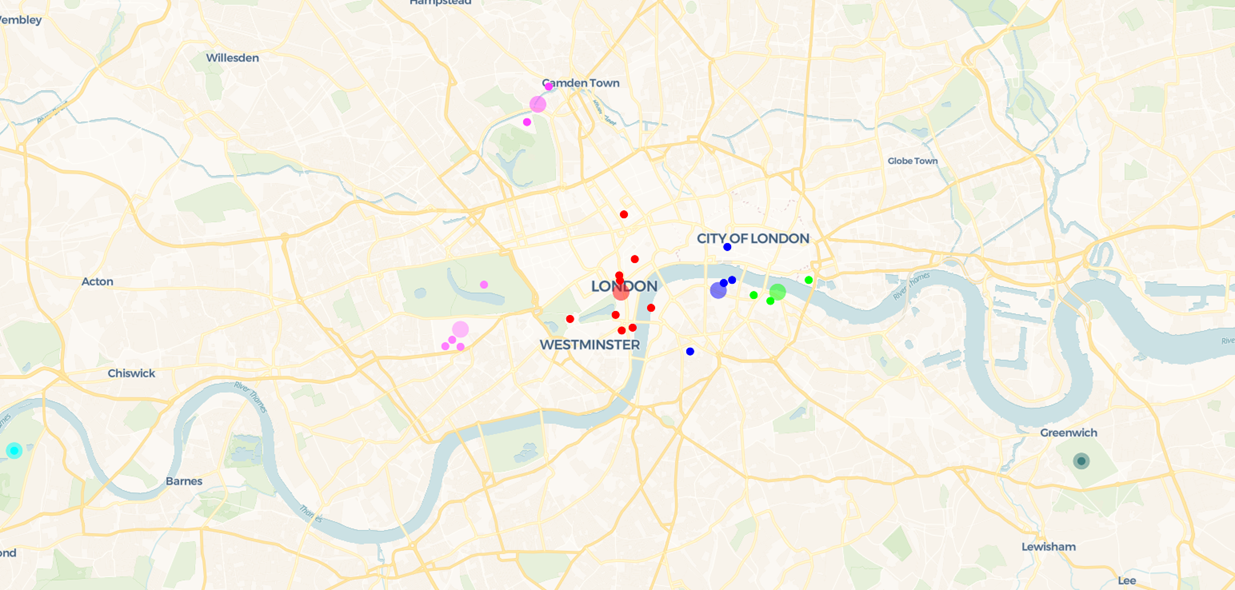
\includegraphics[width = \textwidth]{KMeans_London_Step4}
    \caption{Step4, Centroids have updated and no locations have changed cluster, a solution has been found.}
\end{figure}

\noindent
It is worth noting that K-Means only forms these clusters based on Euclidean distances, grouping together locations
that are close geographically.
However, as formally described in the \hyperref[subsec:objective-function]{Objective Function} section of the
\hyperref[sec:problem-formulation]{Problem Formulation}, a good trip will minimise both the route length of the trip
and the variance between time spent each day.
K-Means does not aim to optimise for the variance between days, it doesn't even consider the time spent at each
location.
Furthermore, while each cluster might be optimised for distance, how close two locations are may not reflect the travel
time between them.
While K-Means does not intentionally optimise for variance between days or consider travel time between locations, it
was still chosen for this project out of curiosity as to how effective a heuristic it might provide.
Hopefully it will offer a simple and computationally efficient baseline for comparison with more complex
algorithms.

\subsubsection{Genetic Clustering}
\todo{Explain genetic clustering}
Genetic clustering applies genetic algorithms to attempt and find the best assignment of locations to clusters.
Genetic algorithms are a type of evolutionary algorithm that aims to mimic biological evolution to find an optimal
solution.
They involve creating a population of potential solutions (individuals) and iteratively improving the population
through selection (keeping the best individuals in the population, akin to natural selection), crossover (combining
individuals to create offspring, akin to sexual reproduction), and mutation (randomly altering the genomes
of individuals in the population, akin to biological mutation).

For us to perform selection, and find the best solutions in a population, we need to assign some fitness to each
individual.
To do this we will combine the cluster assignments with a chosen routing algorithm, and then apply our cost function
to the route found.
This cost will be used to rank our population, helping us find clusters that can produce a good trip.

The performance of Genetic algorithms is highly dependent on its hyperparameters: mutation rate, determining how
common mutation is; crossover rate, determining how often offspring are created via crossover, as opposed to new
additions to the population; population size, determining how many individuals there are per generation; number of
generations, determining how many generations will be evolved to reach a solution; crossover method used,
determining how crossover is performed to create offspring; and in our case, the routing algorithm used, which may
impact how clusters are used to form routes.
These hyperparameters impact both the runtime of the algorithm and the exploration of the search space, indirectly
impacting the quality of the solution.
The time complexity of genetic clustering largely depends on the chosen routing algorithm, b
Genetic clustering has a time complexity of $O(gpn)$, with $g$ being the number of generations, $p$ being the
population size and $n$ being the number of locations.\\

\noindent
For this genetic clustering, an individual is represented by a genome, which will provide a mapping that assigns each
location to a cluster, for example:
\begin{figure}[H]\label{fig:barcelona-genome-example}
    \centering
    Genome: [0, 0, 0, 1, 1, 1, 2, 2, 2]\\
    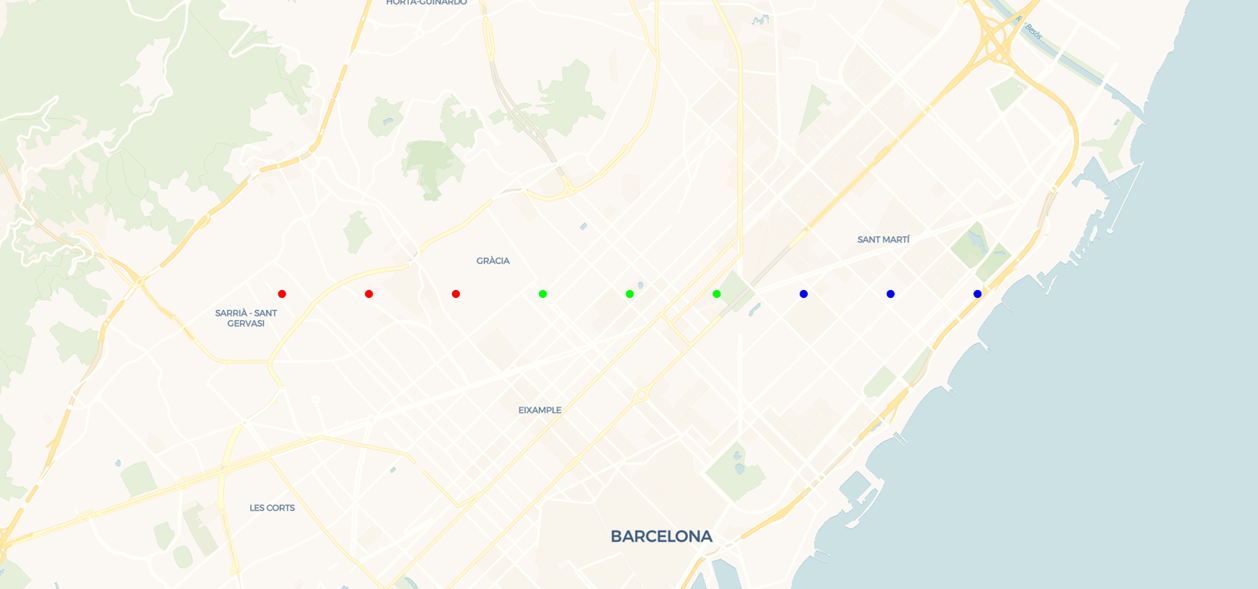
\includegraphics[width = \textwidth]{Barcelona_Genome_Example}
    \caption{An example of how a genome corresponds to cluster assignments.}
\end{figure}

\noindent
These genomes are our target for performing crossover and mutations.
We begin our evolution process by randomly generating an initial population of individuals.
From there, we repeat the following steps until we reach a maximum number of generations:
\begin{enumerate}
    \item Evaluate the fitness of each individual in the population.
    \item Select the best individuals from the population, these will be carried over into the next generation, as
    well as be used to create offspring.
    \item Generate new population using crossover and mutation.
\end{enumerate}

\noindent
As previously discussed, we will evaluate the fitness of each individual by applying a routing algorithms to the
clusters defined by the genome, and then applying our cost function to the resulting route.
Once the population has been evaluated, the best two individuals are chosen as parents.
\begin{figure}[H]\label{fig:Genetic_Clustering.find_clusters.select_parents}
    \centering
    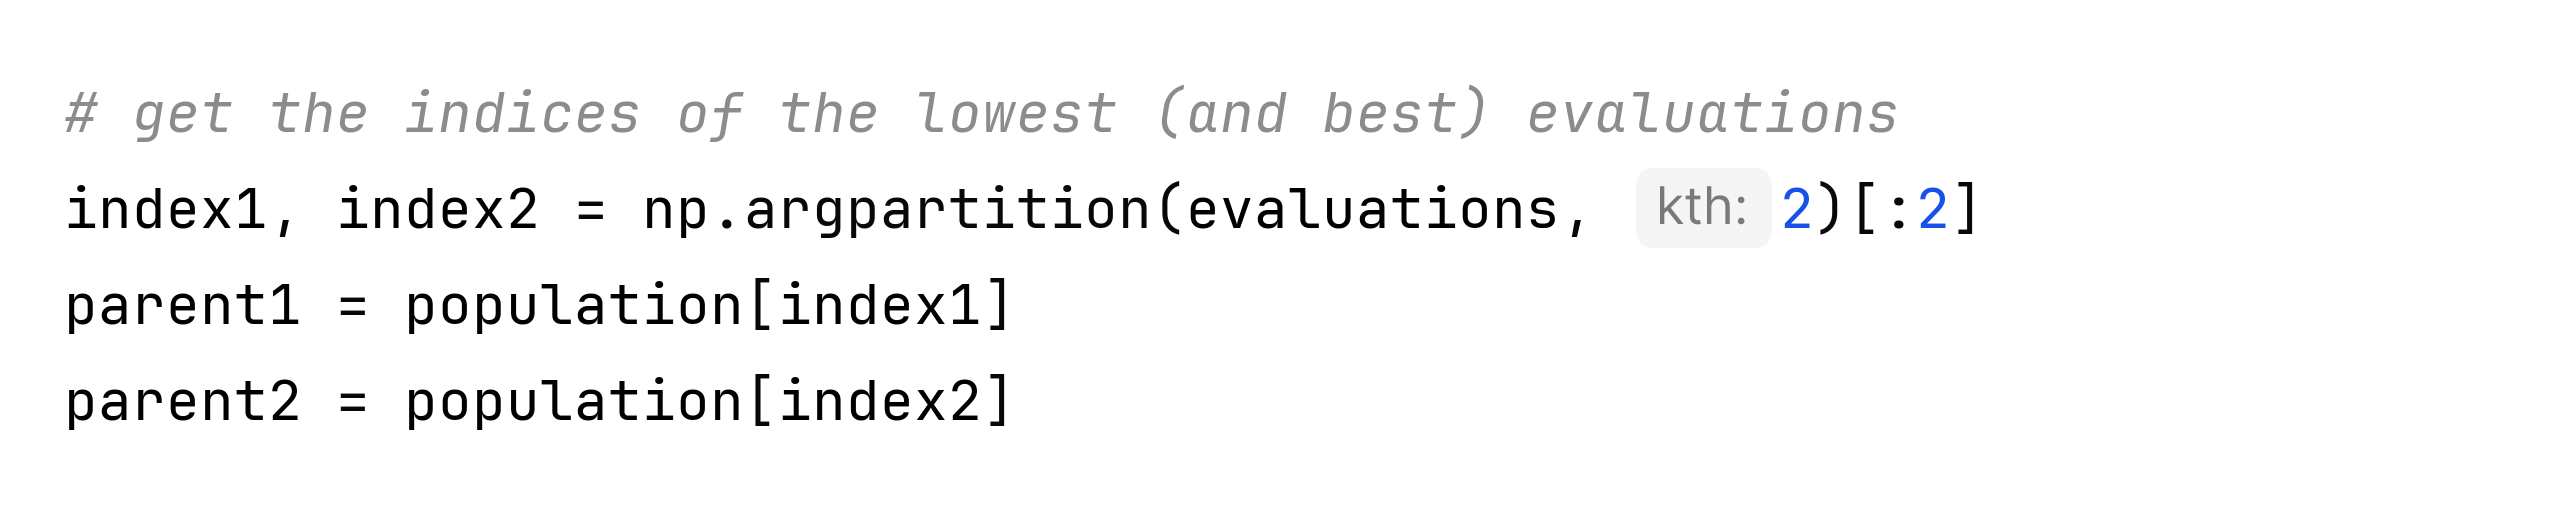
\includegraphics[width = \textwidth]{GeneticClustering.find_clusters.select_parents}
    \caption{from Genetic\_Clustering.find\_clusters in algorithms\textbackslash genetic.py}
\end{figure}

\noindent
Excluding the two parents, who will be copied over, most of the next generation will be created using crossover.
We do however, include some randomly generated individuals, in an effort to increase genetic diversity and
exploration of the search space.
\begin{figure}[H]\label{fig:GeneticClustering.find_clusters.crossover}
    \centering
    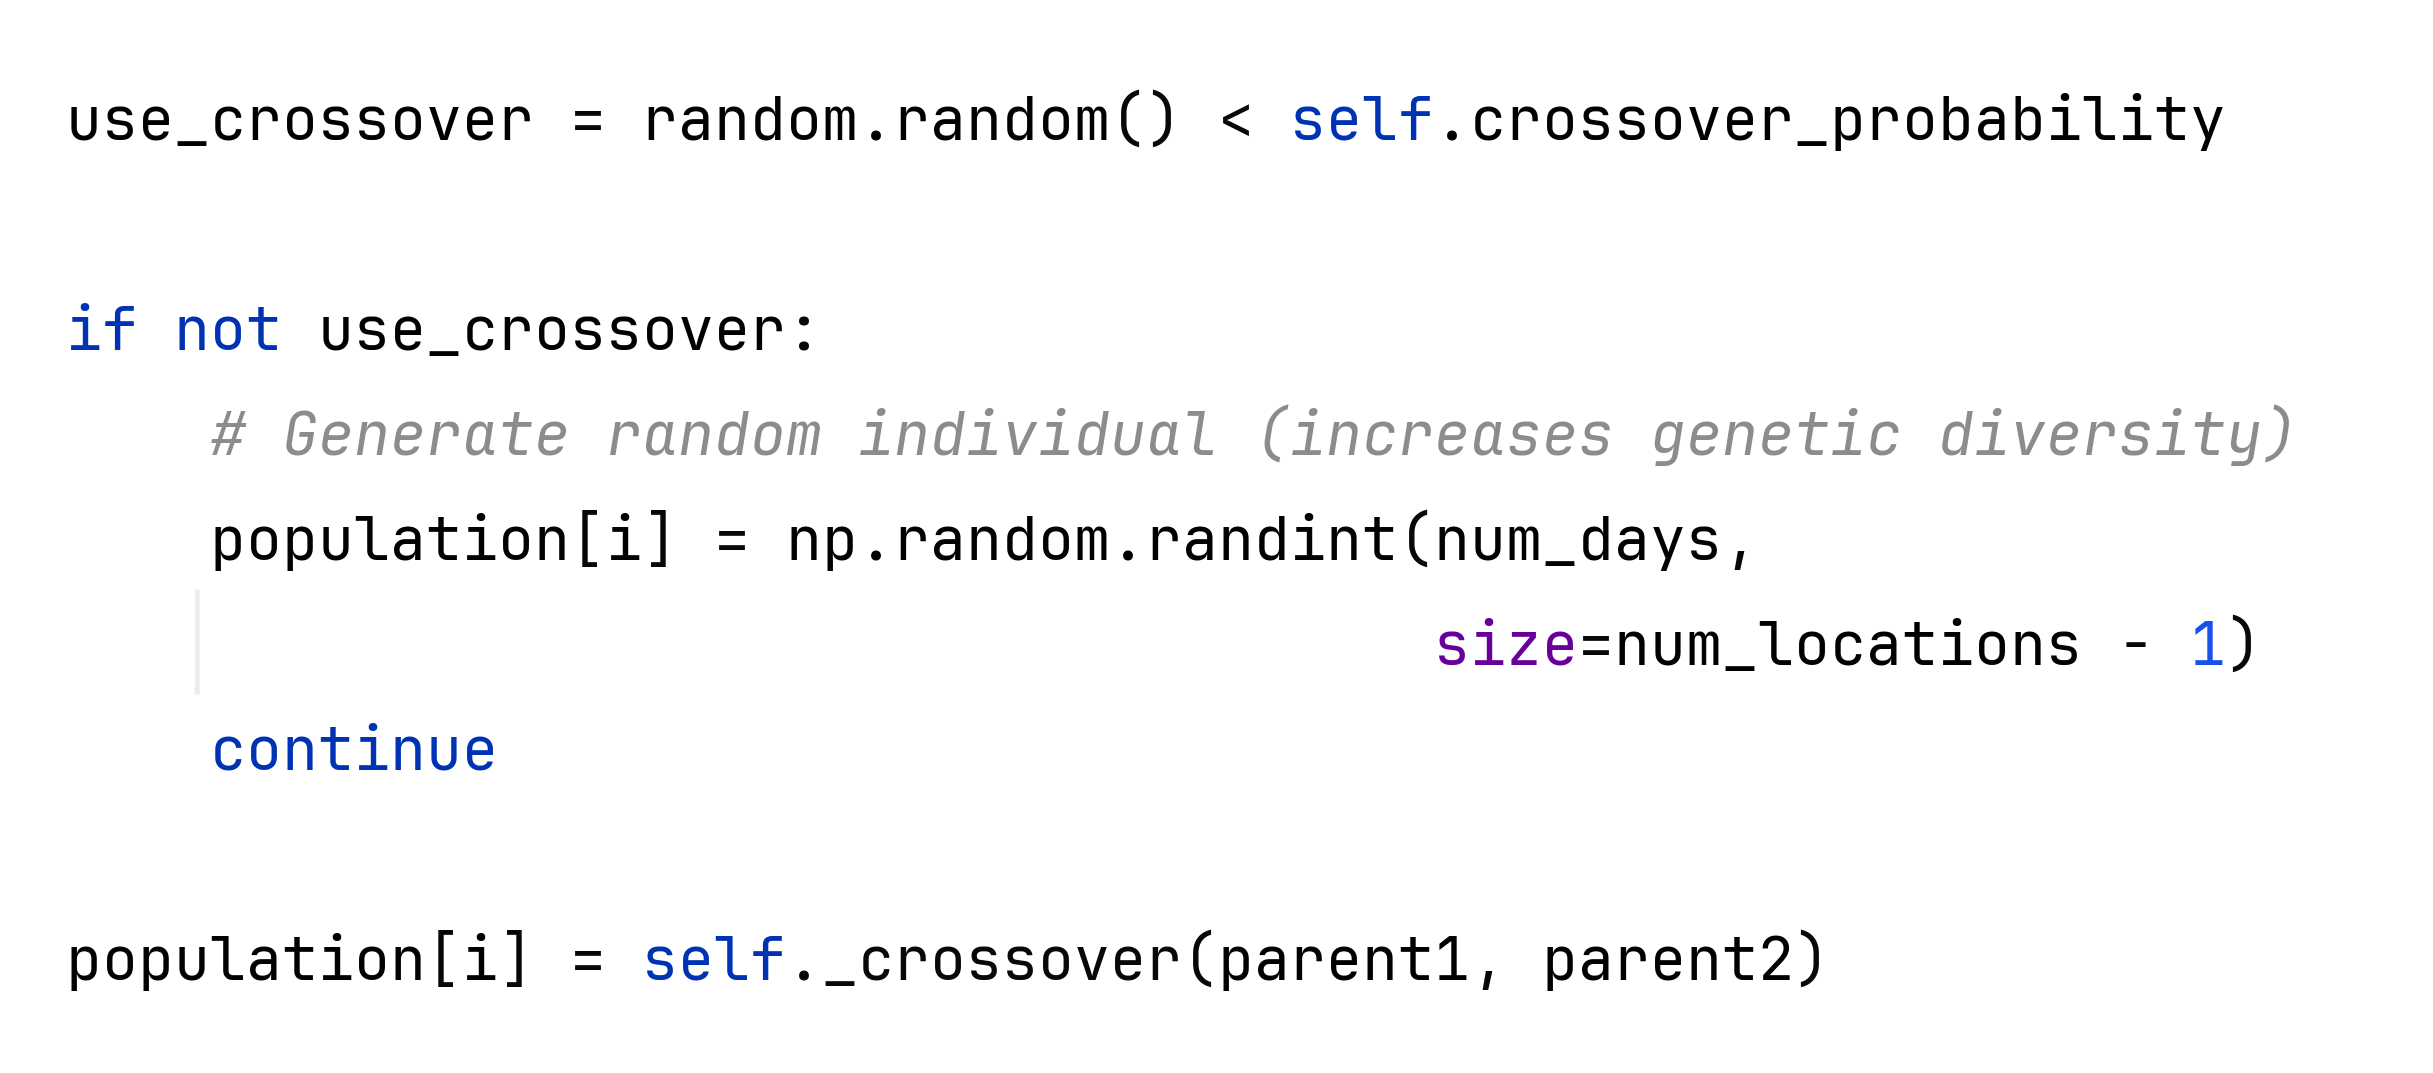
\includegraphics[width = \textwidth]{GeneticClustering.find_clusters.crossover}
    \caption{from Genetic\_Clustering.find\_clusters in algorithms\textbackslash genetic.py}
\end{figure}

\subsubsection{Genetic Centroid-based Clustering}
\todo{Explain genetic centroid-based clustering and how it differs from general clustering.}

\subsection{Routing}\label{subsec:routing}
\todo{Explain purpose of routing/goal of algorithms.}
\subsubsection{Brute Force}\label{subsubsec:brute-force-routing}
\todo{Write brute force explanation}
The brute force algorithm is an exhaustive algorithm that tries every possible route to find one with the least cost.
By checking every route it is guaranteed to find the optimal route, however, its computational cost becomes
impractical as input size grows, having a time complexity of $O(n!)$.\todo{Maybe cite time complexity of brute force?}
Considering we will be comparing algorithms based on their speed and the quality of their results, brute force is a
useful benchmark, providing a lower bound for speed and an upper bound for quality.\\
\\
In our brute force implementation, where n is the number of locations in the route, we will be generating all $n-1!$
permutations of the set $\{1, 2, \mathellipsis, n-1\}$, with each permutation representing the order of locations
visited in a route.
Each route will be evaluated according to our optimisation function, and the route with the lowest cost will be
returned.
We only need to consider $n-1!$ permutations because all our routes will start and end at the same location.\\


\subsubsection{Greedy Routing}\label{subsubsec:greedy-routing}
\todo{Explain greedy routing algorithm}
Greedy routing
\subsubsection{Gift Wrapping}\label{subsubsec:gift-wrapping}
\todo{Explain gift wrapping algorithm}
\todo{Something like: "Once gift wrapping has found a convex hull, a greedy insertion algorithm is used to find the optimal route within the convex hull."}
\subsubsection{Genetic Routing}
\todo{Explain genetic routing}

\subsection{Route Insertion}\label{subsec:route-insertion}
\todo{Explain route insertion, how it is used in route planning and the goal of our algorithms.}
\subsubsection{Brute Force}\label{subsubsec:brute-force-route-insertion}
\todo{Explain how brute force algorithm can be modified for route insertion.}
\subsubsection{Greedy Insertion}\label{subsubsec:greedy-insertion}
\todo{Explain how greedy algorithm can be modified for route insertion.}

\subsection{Trip Generation}\label{subsec:trip-generation}
\todo{Explain trip generation, how it is used in route planning and the goal of our algorithms.}
\subsubsection{Brute Force}\label{subsubsec:brute-force-trip-generation}
\todo{Explain how brute force algorithm can be modified for trip generation.}
\subsubsection{Genetic Trip Generation}
\todo{Explain genetic trip generation}